\documentclass[]{beamer}
\mode<presentation>{
  %% \usetheme[compress]{Berlin}
}
%% packages
\usepackage{zhspacing}
\zhspacing
\usepackage{graphics}
\usepackage{listings}
\lstset{
  basicstyle=\ttfamily\tiny,
  numbers=left
}
\usepackage{tabularx}
\usepackage{booktabs}
%% meta info
\title{Breadth-First Search on Massive Parallel Processing Architectures}
\subtitle{Special Topic on BFS (2)}
\author[SuXing~pysuxing@gmail.com]{SuXing}
\institute{TOW}
\date{\today}

\setbeamercolor{footcolor}{fg=blue,bg=white} % 设置字体和背景颜色
\setbeamertemplate{footline}{%
  \leavevmode%
  \hbox{%
    \begin{beamercolorbox}[wd=.126\paperwidth,ht=2.25ex,dp=1ex,right]{footcolor}%      
       \insertframenumber{} / \inserttotalframenumber\hspace*{5ex}
    \end{beamercolorbox}}%
  \vskip0pt%
}

%% slides
\begin{document}
\setlength{\parindent}{0pt}

\frame{\titlepage}
\frame{\tableofcontents}

\section{Background (Review)}
\frame{\tableofcontents[currentsection]}

\begin{frame}
  \frametitle{Representation of BFS Result}
  Typically, BFS Result could have two forms of representation
  \begin{itemize}
    \item Parent Array (P)
    \item Depth Array (D)
  \end{itemize}
  An implementation could use either or both. e.g. The graph500 benchmark
  uses the Parent Array form
\end{frame}

\begin{frame}
  \frametitle{The BFS Algorithm}
  \begin{figure}
    \centering
    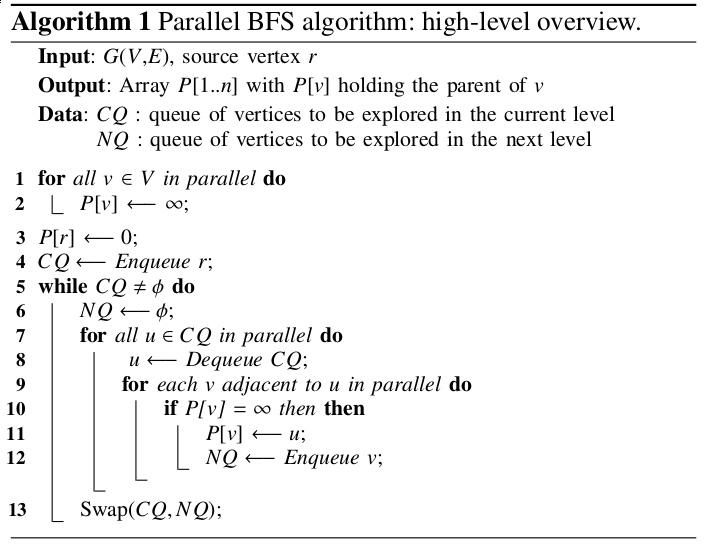
\includegraphics[width=.8\textwidth]{figures/bfs-serial}
  \end{figure}
\end{frame}

\begin{frame}
  \frametitle{Parallelization}
  \begin{itemize}
    \item The parallelism lies in the for loop on line 7, all vertices in CQ
      are partitioned among compute nodes
    \item CQ, NQ and P are also distributed to compute nodes, updating is
      accomplished by explicit communication between compute nodes
  \end{itemize}
  \begin{figure}
    \centering
    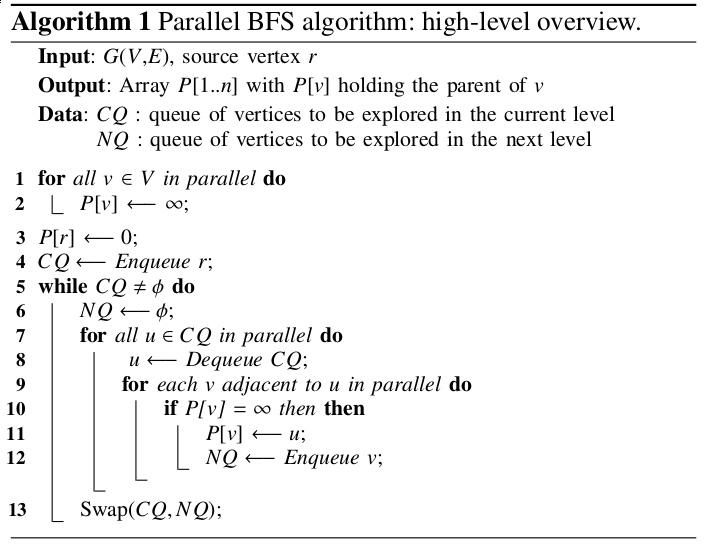
\includegraphics[width=.5\textwidth]{figures/bfs-serial}
  \end{figure}
\end{frame}

\section{Implementation on MPP Architectures}
\frame{\tableofcontents[currentsection]}

\begin{frame}
  \frametitle{Proposed Implementation Techniques}
  Here we show implementation techniques proposed by several papers
  \begin{itemize}
    \item A Scalable Distributed Parallel Breadth-First Search Algorithm on BlueGene/L (SC'05)
    \item Parallel Breadth-first Search on Distributed Memory Systems (SC'11)
    \item Direction-Optimizing Breadth-First Search (SC'12)
    \item Large-Scale Energy-Efficient Graph Traversal A Path to Efficient Data-Intensive Supercomputing (SC'12)
  \end{itemize}
\end{frame}

\subsection{Graph Partitioning}
\frame{\tableofcontents[currentsection, currentsubsection]}

\begin{frame}
  \frametitle{1-D Partitioning}
  The 1-D partitioning method is vertex-centric. It distributes all vertices among
  compute nodes, along with its outgoing edges.
  \begin{itemize}
    \item Every compute node owns a chunk of vertices exclusively
    \item The partitioning logic is simple and straitforward\\
      e.g. $Owner(v) = v \mod NumOfComputeNodes$
    \item All-to-all communication is needed in each search iteration
  \end{itemize}
\end{frame}

\begin{frame}
  \frametitle{2-D Partitioning}
  The 2-D partitioning method is combination of edge- and vertex-centric.
  Both edges and vertices are distributed among compute nodes.
  The adjacency matrix is paritioned into
  $RC \times C$ blocks, and processes are arranged as a $R \times C$ matrix, mappings of edges and vertices
  to processes is shown in red and blue arrows, respectively
  \begin{figure}
    \includegraphics[width=.4\textwidth]{figures/sc05-graph}
    \caption{2-D partitioning of the adjacency matrix}
  \end{figure}
\end{frame}

\begin{frame}
  \frametitle{Advantages of 2-D Partitioning}
  The 2-D partitioning method was originally proposed by \cite{Yoo2005}, and 
  and many other researchers has designed BFS algorithms based on it,
  including \cite{Bulucc2011}.

  Compared to 1-D partitioning, the 2-D partitioning
  method convert global all-to-all communications to subgroup (column-wise and
  row-wise) collective communications, thus elimating communication overhead.  
\end{frame}

\subsection{Bidirectional Search}
\frame{\tableofcontents[currentsection, currentsubsection]}

\begin{frame}
  \frametitle{Top-down Search: the Traditional Way}
  In traditional BFS algorithms, searching always starts from the souce vertex
  and goes down to the deepest vertices. When performed on MPP architectures,
  this will cause large amout of unnecessary communication.
  \begin{block}{Insight}
    As the search going on, the frontier may grow to contain large number of vertices,
    and expanding this frontier will cause a lot of visited vertices to be re-visited.
  \end{block}
\end{frame}

\begin{frame}
  \frametitle{Neigbors Breakdown in Search Iterations}
  This figure shows the expanded neigbors breakdwon in each iteration.
  We can see that most of the work is unnecessary, which means most of
  the communication is useless!
  \begin{figure}
    \includegraphics[width=.7\textwidth]{figures/sc12-bidirectional}
  \end{figure}
\end{frame}

\begin{frame}
  \frametitle{Solution: Bidirectional Search}
  \cite{Beamer2012} proposed a bidirectional method which combine traditional top-down
  method and a innovative bottom-up method.
  \begin{itemize}
    \item At the beginning of BFS, searching is performed in top-down way
    \item When the frontier is large enough, searching is swithed to the bottom-up way
    \item When the frontier starts to shrink, searching direction is switched back.
  \end{itemize}
  \begin{figure}
    \includegraphics[width=.5\textwidth]{figures/sc12-states}
  \end{figure}
\end{frame}

%% \subsection{Compression Based Communication Optimizations}
%% \frame{\tableofcontents[currentsection, currentsubsection]}

%% \begin{frame}
%%   \frametitle{}
%% \end{frame}

\section{Summary}
\frame{\tableofcontents[currentsection]}

\begin{frame}
  \frametitle{Summary}
  Algorithm design on MPP architectures
  \begin{itemize}
    \item 2-D graph partitioning
    \item Bidirectional searching
  \end{itemize}
\end{frame}

\begin{frame}
  \frametitle{References}
  \bibliographystyle{plain}
  \bibliography{refs.bib}
\end{frame}

\frame{\centerline{\Huge Q\&A}}

\end{document}
